% Commutative diagram with edges passing under/over
% Jan 7, 2009, Stefan Kottwitz
% http://texblog.net
\documentclass[class=minimal,border=0pt]{article}
\usepackage{tikz}
\usepackage[paperwidth=10cm,paperheight=7.5cm,hmargin=0.4cm,vmargin=0.5cm]{geometry}
\usetikzlibrary{matrix}

\begin{document}

\begin{tikzpicture}

% define feature map parameters
\pgfmathsetmacro{\cubex}{0.1}
\pgfmathsetmacro{\cubey}{4}
\pgfmathsetmacro{\cubez}{5}
\pgfmathsetmacro{\multx}{0.9}
\pgfmathsetmacro{\divyz}{1.7}

\pgfmathsetmacro{\x}{0}

% offset between the feature maps
\pgfmathsetmacro{\offset}{0.12}

% perspective parameter
\pgfmathsetmacro{\xx}{0.5}

% define color
\definecolor{convfill}{RGB}{255,255,255}
\definecolor{convline}{RGB}{0,0,0}

\definecolor{maxline}{RGB}{255,0,0}
\definecolor{maxfill}{RGB}{255,255,255}

\definecolor{fcfill}{RGB}{255,255,255}
\definecolor{fcline}{RGB}{6,185,251}

\definecolor{softmaxfill}{RGB}{255,255,255}
\definecolor{softmaxline}{RGB}{191,115,16}

\definecolor{colorarrow}{RGB}{0,0,205}

% input image
\node[inner sep=0pt,cm={0.35 ,0.5 ,0 ,1  ,(0 cm,0 cm)}] (image) at (-1,0)
    {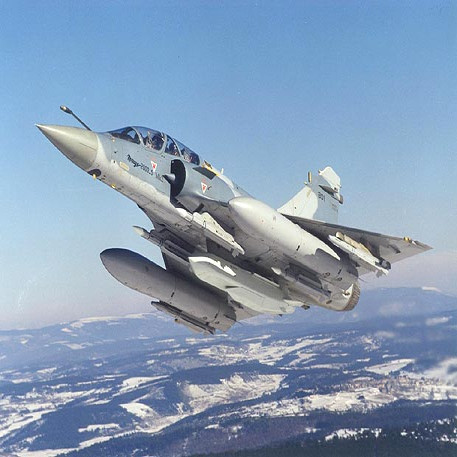
\includegraphics[width=\cubey cm]{images/mirage2000}};
   
\node[text width=3cm] at (\x+\xx/2-\xx-0.8,\cubey/2+0.12,\cubez/2-\cubez) {\scriptsize $224 \! \times \! 224 \! \times \! 3$};

\pgfmathsetmacro{\cubey}{\cubey/1.5}
\pgfmathsetmacro{\cubez}{\cubez/1.5}
\pgfmathsetmacro{\xx}{\xx/1.5}

%% conv1
\draw[convline,fill=convfill] (\x+\xx/2,\cubey/2,\cubez/2) -- ++(-\cubex,0,0) -- ++(0,-\cubey,0) -- ++(\cubex,0,0) -- cycle;
\draw[convline,fill=convfill] (\x+\xx/2,\cubey/2,\cubez/2) -- ++(0-\xx,0,-\cubez) -- ++(0,-\cubey,0) -- ++(0+\xx,0,\cubez) -- cycle;
\draw[convline,fill=convfill] (\x+\xx/2,\cubey/2,\cubez/2) -- ++(-\cubex,0,0) -- ++(0-\xx,0,-\cubez) -- ++(\cubex,0,0) -- cycle;

\node[text width=3cm] at (\x+\xx/2-\xx+1,\cubey/2+0.12,\cubez/2-\cubez) {\scriptsize $109 \! \times \! 109 \! \times \! 96$};

\coordinate (conv1_2) at (\x+\xx/2-\cubex/2,0,\cubez/2);


% pool1
\pgfmathsetmacro{\cubey}{\cubey/\divyz}
\pgfmathsetmacro{\cubez}{\cubez/\divyz}
\pgfmathsetmacro{\x}{\x + \cubex + \offset}
\pgfmathsetmacro{\xx}{\xx/\divyz}
\draw[maxline,fill=maxfill] (\x+\xx/2,\cubey/2,\cubez/2) -- ++(-\cubex,0,0) -- ++(0,-\cubey,0) -- ++(\cubex,0,0) -- cycle;
\draw[maxline,fill=maxfill] (\x+\xx/2,\cubey/2,\cubez/2) -- ++(0-\xx,0,-\cubez) -- ++(0,-\cubey,0) -- ++(0+\xx,0,\cubez) -- cycle;
\draw[maxline,fill=maxfill] (\x+\xx/2,\cubey/2,\cubez/2) -- ++(-\cubex,0,0) -- ++(0-\xx,0,-\cubez) -- ++(\cubex,0,0) -- cycle;

\coordinate (pool1) at (\x+\xx/2-\cubex/2,0,\cubez/2);

\pgfmathsetmacro{\cubey}{\cubey/\divyz}
\pgfmathsetmacro{\cubez}{\cubez/\divyz}
\pgfmathsetmacro{\xx}{\xx/\divyz}

% conv2
\pgfmathsetmacro{\cubex}{\cubex*\multx*2.7}
\pgfmathsetmacro{\x}{\x + \cubex + \offset}
\draw[convline,fill=convfill] (\x+\xx/2,\cubey/2,\cubez/2) -- ++(-\cubex,0,0) -- ++(0,-\cubey,0) -- ++(\cubex,0,0) -- cycle;
\draw[convline,fill=convfill] (\x+\xx/2,\cubey/2,\cubez/2) -- ++(0-\xx,0,-\cubez) -- ++(0,-\cubey,0) -- ++(0+\xx,0,\cubez) -- cycle;
\draw[convline,fill=convfill] (\x+\xx/2,\cubey/2,\cubez/2) -- ++(-\cubex,0,0) -- ++(0-\xx,0,-\cubez) -- ++(\cubex,0,0) -- cycle;

\node[text width=3cm] at (\x+\xx/2-\xx+1,\cubey/2+0.12,\cubez/2-\cubez) {\scriptsize $26 \! \times \! 26 \! \times \! 256$};

\coordinate (conv2_2) at (\x+\xx/2-\cubex/2,0,\cubez/2);

% pool2
\pgfmathsetmacro{\cubey}{\cubey/\divyz}
\pgfmathsetmacro{\cubez}{\cubez/\divyz}
\pgfmathsetmacro{\x}{\x + \cubex + \offset}
\pgfmathsetmacro{\xx}{\xx/\divyz}
\draw[maxline,fill=maxfill] (\x+\xx/2,\cubey/2,\cubez/2) -- ++(-\cubex,0,0) -- ++(0,-\cubey,0) -- ++(\cubex,0,0) -- cycle;
\draw[maxline,fill=maxfill] (\x+\xx/2,\cubey/2,\cubez/2) -- ++(0-\xx,0,-\cubez) -- ++(0,-\cubey,0) -- ++(0+\xx,0,\cubez) -- cycle;
\draw[maxline,fill=maxfill] (\x+\xx/2,\cubey/2,\cubez/2) -- ++(-\cubex,0,0) -- ++(0-\xx,0,-\cubez) -- ++(\cubex,0,0) -- cycle;

\coordinate (pool2) at (\x+\xx/2-\cubex/2,0,\cubez/2);

% conv3
\pgfmathsetmacro{\cubex}{\cubex*\multx*2}
\pgfmathsetmacro{\x}{\x + \cubex + \offset}
\draw[convline,fill=convfill] (\x+\xx/2,\cubey/2,\cubez/2) -- ++(-\cubex,0,0) -- ++(0,-\cubey,0) -- ++(\cubex,0,0) -- cycle;
\draw[convline,fill=convfill] (\x+\xx/2,\cubey/2,\cubez/2) -- ++(0-\xx,0,-\cubez) -- ++(0,-\cubey,0) -- ++(0+\xx,0,\cubez) -- cycle;
\draw[convline,fill=convfill] (\x+\xx/2,\cubey/2,\cubez/2) -- ++(-\cubex,0,0) -- ++(0-\xx,0,-\cubez) -- ++(\cubex,0,0) -- cycle;


% conv4
\pgfmathsetmacro{\cubex}{\cubex*\multx}
\pgfmathsetmacro{\x}{\x + \cubex + \offset}
\draw[convline,fill=convfill] (\x+\xx/2,\cubey/2,\cubez/2) -- ++(-\cubex,0,0) -- ++(0,-\cubey,0) -- ++(\cubex,0,0) -- cycle;
\draw[convline,fill=convfill] (\x+\xx/2,\cubey/2,\cubez/2) -- ++(0-\xx,0,-\cubez) -- ++(0,-\cubey,0) -- ++(0+\xx,0,\cubez) -- cycle;
\draw[convline,fill=convfill] (\x+\xx/2,\cubey/2,\cubez/2) -- ++(-\cubex,0,0) -- ++(0-\xx,0,-\cubez) -- ++(\cubex,0,0) -- cycle;

\node[text width=3cm] at (\x+\xx/2-\xx+0.5,\cubey/2+0.12,\cubez/2-\cubez) {\scriptsize $13 \! \times \! 13 \! \times \! 512$};

% conv5
\pgfmathsetmacro{\x}{\x + \cubex + \offset}
\draw[convline,fill=convfill] (\x+\xx/2,\cubey/2,\cubez/2) -- ++(-\cubex,0,0) -- ++(0,-\cubey,0) -- ++(\cubex,0,0) -- cycle;
\draw[convline,fill=convfill] (\x+\xx/2,\cubey/2,\cubez/2) -- ++(0-\xx,0,-\cubez) -- ++(0,-\cubey,0) -- ++(0+\xx,0,\cubez) -- cycle;
\draw[convline,fill=convfill] (\x+\xx/2,\cubey/2,\cubez/2) -- ++(-\cubex,0,0) -- ++(0-\xx,0,-\cubez) -- ++(\cubex,0,0) -- cycle;


% pool5
\pgfmathsetmacro{\cubey}{\cubey/2}
\pgfmathsetmacro{\cubez}{\cubez/2}
\pgfmathsetmacro{\x}{\x + \cubex + \offset}
\pgfmathsetmacro{\xx}{\xx/\divyz}
\draw[maxline,fill=maxfill] (\x+\xx/2,\cubey/2,\cubez/2) -- ++(-\cubex,0,0) -- ++(0,-\cubey,0) -- ++(\cubex,0,0) -- cycle;
\draw[maxline,fill=maxfill] (\x+\xx/2,\cubey/2,\cubez/2) -- ++(0-\xx,0,-\cubez) -- ++(0,-\cubey,0) -- ++(0+\xx,0,\cubez) -- cycle;
\draw[maxline,fill=maxfill] (\x+\xx/2,\cubey/2,\cubez/2) -- ++(-\cubex,0,0) -- ++(0-\xx,0,-\cubez) -- ++(\cubex,0,0) -- cycle;

\node[text width=3cm] (sizepool5) at (\x+\xx/2-\xx+0.8,\cubey/2+0.8,0) {\scriptsize $6 \! \times \! 6 \! \times \! 512$};

\draw[-stealth] (\x+\xx/2-\xx -\cubex/2,\cubey/2+0.7,0)--(\x+\xx/2-\xx -\cubex/2,\cubey/2 ,0);

\coordinate (pool5) at (\x+\xx/2-\cubex/2,0,\cubez/2);

% fc6
\pgfmathsetmacro{\cubex}{\cubex*2.5}
\pgfmathsetmacro{\cubey}{\cubey/3}
\pgfmathsetmacro{\cubez}{\cubez/3}
\pgfmathsetmacro{\x}{\x + \cubex + \offset}
\pgfmathsetmacro{\xx}{\xx/\divyz}
\draw[fcline,fill=fcfill] (\x+\xx/2,\cubey/2,\cubez/2) -- ++(-\cubex,0,0) -- ++(0,-\cubey,0) -- ++(\cubex,0,0) -- cycle;
\draw[fcline,fill=fcfill] (\x+\xx/2,\cubey/2,\cubez/2) -- ++(0-\xx,0,-\cubez) -- ++(0,-\cubey,0) -- ++(0+\xx,0,\cubez) -- cycle;
\draw[fcline,fill=fcfill] (\x+\xx/2,\cubey/2,\cubez/2) -- ++(-\cubex,0,0) -- ++(0-\xx,0,-\cubez) -- ++(\cubex,0,0) -- cycle;

\coordinate (fc6) at (\x+\xx/2-\cubex/2,0,\cubez/2);

% fc7
\pgfmathsetmacro{\x}{\x + \cubex + \offset}
\draw[fcline,fill=fcfill] (\x+\xx/2,\cubey/2,\cubez/2) -- ++(-\cubex,0,0) -- ++(0,-\cubey,0) -- ++(\cubex,0,0) -- cycle;
\draw[fcline,fill=fcfill] (\x+\xx/2,\cubey/2,\cubez/2) -- ++(0-\xx,0,-\cubez) -- ++(0,-\cubey,0) -- ++(0+\xx,0,\cubez) -- cycle;
\draw[fcline,fill=fcfill] (\x+\xx/2,\cubey/2,\cubez/2) -- ++(-\cubex,0,0) -- ++(0-\xx,0,-\cubez) -- ++(\cubex,0,0) -- cycle;

\node[text width=3cm] at (\x+\xx/2-\xx-0.1,\cubey/2+0.12,\cubez/2-\cubez) {\scriptsize $1 \! \times \! 1 \! \times \! 4096$};

% fc8
\pgfmathsetmacro{\cubex}{\cubex/2}
\pgfmathsetmacro{\x}{\x + \cubex + \offset}
\draw[fcline,fill=fcfill] (\x+\xx/2,\cubey/2,\cubez/2) -- ++(-\cubex,0,0) -- ++(0,-\cubey,0) -- ++(\cubex,0,0) -- cycle;
\draw[fcline,fill=fcfill] (\x+\xx/2,\cubey/2,\cubez/2) -- ++(0-\xx,0,-\cubez) -- ++(0,-\cubey,0) -- ++(0+\xx,0,\cubez) -- cycle;
\draw[fcline,fill=fcfill] (\x+\xx/2,\cubey/2,\cubez/2) -- ++(-\cubex,0,0) -- ++(0-\xx,0,-\cubez) -- ++(\cubex,0,0) -- cycle;

% softmax
\pgfmathsetmacro{\x}{\x + \cubex + \offset}
\draw[softmaxline,fill=softmaxfill] (\x+\xx/2,\cubey/2,\cubez/2) -- ++(-\cubex,0,0) -- ++(0,-\cubey,0) -- ++(\cubex,0,0) -- cycle;
\draw[softmaxline,fill=softmaxfill] (\x+\xx/2,\cubey/2,\cubez/2) -- ++(0-\xx,0,-\cubez) -- ++(0,-\cubey,0) -- ++(0+\xx,0,\cubez) -- cycle;
\draw[softmaxline,fill=softmaxfill] (\x+\xx/2,\cubey/2,\cubez/2) -- ++(-\cubex,0,0) -- ++(0-\xx,0,-\cubez) -- ++(\cubex,0,0) -- cycle;

\node[text width=3cm] at (\x+\xx/2-\xx+0.3,\cubey/2+0.12,\cubez/2-\cubez) {\scriptsize $1 \! \times \! 1 \! \times \! 1000$};

\pgfmathsetmacro{\x}{\x/2}
\pgfmathsetmacro{\y}{-1.2}
\pgfmathsetmacro{\cubex}{\cubex/1.5}
\pgfmathsetmacro{\cubey}{\cubey*1.5}
\pgfmathsetmacro{\cubez}{\cubez*1.5}

\draw[convline,fill=convfill] (\x+\xx/2,\y+\cubey/2,\cubez/2) -- ++(-\cubex,0,0) -- ++(0,-\cubey,0) -- ++(\cubex,0,0) -- cycle;
\draw[convline,fill=convfill] (\x+\xx/2,\y+\cubey/2,\cubez/2) -- ++(0-\xx,0,-\cubez) -- ++(0,-\cubey,0) -- ++(0+\xx,0,\cubez) -- cycle;
\draw[convline,fill=convfill] (\x+\xx/2,\y+\cubey/2,\cubez/2) -- ++(-\cubex,0,0) -- ++(0-\xx,0,-\cubez) -- ++(\cubex,0,0) -- cycle;

\node[text width=3cm] at (\x+1.7,\y+0.05,0) {\scriptsize convolution+ReLU};

\pgfmathsetmacro{\y}{\y-0.35}
\draw[maxline,fill=maxfill] (\x+\xx/2,\y+\cubey/2,\cubez/2) -- ++(-\cubex,0,0) -- ++(0,-\cubey,0) -- ++(\cubex,0,0) -- cycle;
\draw[maxline,fill=maxfill] (\x+\xx/2,\y+\cubey/2,\cubez/2) -- ++(0-\xx,0,-\cubez) -- ++(0,-\cubey,0) -- ++(0+\xx,0,\cubez) -- cycle;
\draw[maxline,fill=maxfill] (\x+\xx/2,\y+\cubey/2,\cubez/2) -- ++(-\cubex,0,0) -- ++(0-\xx,0,-\cubez) -- ++(\cubex,0,0) -- cycle;

\node[text width=3cm] at (\x+1.7,\y+0.05,0) {\scriptsize max pooling};

\pgfmathsetmacro{\y}{\y-0.35}
\draw[fcline,fill=fcfill] (\x+\xx/2,\y+\cubey/2,\cubez/2) -- ++(-\cubex,0,0) -- ++(0,-\cubey,0) -- ++(\cubex,0,0) -- cycle;
\draw[fcline,fill=fcfill] (\x+\xx/2,\y+\cubey/2,\cubez/2) -- ++(0-\xx,0,-\cubez) -- ++(0,-\cubey,0) -- ++(0+\xx,0,\cubez) -- cycle;
\draw[fcline,fill=fcfill] (\x+\xx/2,\y+\cubey/2,\cubez/2) -- ++(-\cubex,0,0) -- ++(0-\xx,0,-\cubez) -- ++(\cubex,0,0) -- cycle;

\node[text width=3cm] at (\x+1.7,\y+0.05,0) {\scriptsize fully connected+ReLU};

\pgfmathsetmacro{\y}{\y-0.35}
\draw[softmaxline,fill=softmaxfill] (\x+\xx/2,\y+\cubey/2,\cubez/2) -- ++(-\cubex,0,0) -- ++(0,-\cubey,0) -- ++(\cubex,0,0) -- cycle;
\draw[softmaxline,fill=softmaxfill] (\x+\xx/2,\y+\cubey/2,\cubez/2) -- ++(0-\xx,0,-\cubez) -- ++(0,-\cubey,0) -- ++(0+\xx,0,\cubez) -- cycle;
\draw[softmaxline,fill=softmaxfill] (\x+\xx/2,\y+\cubey/2,\cubez/2) -- ++(-\cubex,0,0) -- ++(0-\xx,0,-\cubez) -- ++(\cubex,0,0) -- cycle;

\node[text width=3cm] at (\x+1.7,\y+0.05,0) {\scriptsize softmax};

\pgfmathsetmacro{\linesize}{1}


\end{tikzpicture}

\end{document}
